\documentclass[12pt,a4paper,openany]{book}
\usepackage{lmodern}
\usepackage[table]{xcolor}
\input{/home/aroquemaurel/cours/includesLaTeX/couleurs.tex}

\usepackage[utf8]{inputenc} \usepackage[T1]{fontenc}
\usepackage[francais]{babel}
\usepackage[top=1.7cm, bottom=1.7cm, left=1.7cm, right=1.7cm]{geometry}
\usepackage{verbatim}
\usepackage[urlbordercolor={1 1 1}, linkbordercolor={1 1 1}, linkcolor=vert1, urlcolor=bleu, colorlinks=true]{hyperref}
\usepackage{tikz} %Vectoriel
\usepackage{listings}
\usepackage{fancyhdr}
\usepackage{multido}
\usepackage{float}
\usepackage{amssymb}
\usepackage{longtable}
\usepackage{wrapfig}

\newcommand{\titre}{Conception d'une application de folksonomies}

\newcommand{\pole}{}
\newcommand{\sigle}{siaweb}

\newcommand{\semestre}{4}

\input{/home/aroquemaurel/cours/includesLaTeX/listings.tex}
\date{\today}

\makeindex
\lfoot{Université Toulouse III -- Paul Sabatier}
\rfoot{}
%\rfoot{}
\cfoot{}
\makeglossary
\makeatletter
\def\clap#1{\hbox to 0pt{\hss #1\hss}}%
\def\ligne#1{%
\hbox to \hsize{%
\vbox{\centering #1}}}%
\def\haut#1#2#3{%
\hbox to \hsize{%
\rlap{\vtop{\raggedright #1}}%
\hss
\clap{\vtop{\centering #2}}%
\hss
\llap{\vtop{\raggedleft #3}}}}%
\def\bas#1#2#3{%
\hbox to \hsize{%
\rlap{\vbox{\raggedright #1}}%
\hss \clap{\vbox{\centering #2}}%
\hss
\llap{\vbox{\raggedleft #3}}}}%
\def\maketitle{%
\thispagestyle{empty}\vbox to \vsize{%
\haut{}{\@blurb}{}

\vfill
\vspace{1cm}
\begin{flushleft}
\usefont{OT1}{ptm}{m}{n}
\huge \@title
\end{flushleft}
\par
\hrule height 4pt
\par
\begin{flushright}
\usefont{OT1}{phv}{m}{n}
\Large \@author
\par
\end{flushright}
\vspace{1cm}
\vfill
\vfill
\bas{}{\@location, le \@date}{}
}%
\cleardoublepage
}
\def\date#1{\def\@date{#1}}
\def\author#1{\def\@author{#1}}
\def\title#1{\def\@title{#1}}
\def\location#1{\def\@location{#1}}
\def\blurb#1{\def\@blurb{#1}}
\date{\today}
\author{}
\title{}
\location{Amiens}\blurb{}
\makeatother
\title{\titre}
\author{Systèmes d'information et applications Web}

\location{Toulouse}
\blurb{%
Université Toulouse III -- Paul sabatier\\
L2 Informatique\\
\vspace{30px}
\begin{flushleft}Antoine de \bsc{Roquemaurel} (\texttt{\href{mailto:antoine.de-roquemaurel@univ-tlse3.fr}{antoine.de-roquemaurel@univ-tlse3.fr}})\\ 
 Groupe 2.2\end{flushleft}
}%



%\title{Cours \\ \titre}
%\date{\today\\ Semestre \semestre}

%\lhead{Cours: \titre}
%\chead{}
%\rhead{\thepage}

%\lfoot{Université Paul Sabatier Toulouse III}
%\cfoot{\thepage}
%\rfoot{\sigle\semestre}

\pagestyle{fancy}
\renewcommand{\chaptermark}[1]{\markboth{\bsc{\chaptername~\thechapter{} :} #1}{}}
\renewcommand{\sectionmark}[1]{\markright{\thesection{ #1}}}
\renewcommand{\headrulewidth}{0.3pt}
\renewcommand{\footrulewidth}{0.3pt}

\fancyhf{}
\fancyhead[LE]{\leftmark}
\fancyhead[RO]{\rightmark}
\fancyfoot[LE,RO]{--~\thepage~--}
\fancyfoot[LO]{\titre{}}
\fancyfoot[RE]{Antoine de \bsc{Roquemaurel}}

%% Cas des premières pages de chapitre
\fancypagestyle{plain}{%
	\fancyhf{}%
	\fancyfoot[L]{\titre{}}
	\fancyfoot[R]{--~\thepage~--}
	\renewcommand{\headrulewidth}{0pt}
	\renewcommand{\footrulewidth}{0.3pt}
}
\makeatletter
\renewcommand*{\lstlistlistingname}{Liste des codes sources}
\renewcommand\listoffigures{%
    \chapter{\listfigurename}%
      \@mkboth{\MakeUppercase\listfigurename}%
              {\MakeUppercase\listfigurename}%
       \@starttoc{lof}%
    }
    \renewcommand\listoftables{%
    \chapter{\listtablename}%
    \@mkboth{\MakeUppercase{\listtablename}}%
            {\MakeUppercase{\listtablename}}%
    \@starttoc{lot}
    }

    \renewcommand\lstlistoflistings{%
    \begingroup
    \chapter{\lstlistlistingname}%
    \parskip\z@\parindent\z@\parfillskip \z@ \@plus 1fil%
    \@starttoc{lol}%
    \endgroup
    }
	\makeatother

\input{/home/aroquemaurel/cours/includesLaTeX/remarquesExempleAttention.tex}
\input{/home/aroquemaurel/cours/includesLaTeX/polices.tex}
\input{/home/aroquemaurel/cours/includesLaTeX/affichageChapitre.tex}
\let\pagebreakORIG\pagebreak
\let\clearpageORIG\clearpage
\let\cleardoublepageORIG\cleardoublepage

\ifx \removepagebreak \undefined
\newcommand{\removepagebreak}{\renewcommand{\pagebreak}{}\renewcommand{\clearpage}{}\renewcommand{\cleardoublepage}{}}
\fi

\ifx \restorepagebreak \undefined
\newcommand{\restorepagebreak}{\renewcommand{\pagebreak}{\pagebreakORIG}\renewcommand{\clearpage}{\clearpageORIG}\renewcommand{\cleardoublepage}{\cleardoublepageORIG}}
\fi
\newcommand{\pfp}{\texttt{pfp}}

\newcommand{\ifp}{\texttt{if}}
\newcommand{\elsep}{\texttt{else}}

\makeatother
\includeonly {
}
\newcommand{\bootstrap}{\textit{bootstrap}}
\begin{document}
	\setcounter{tocdepth}{2}
	\setcounter{secnumdepth}{3}
	\removepagebreak
	\maketitle
	\newpage
	\chapter*{Avant-propos}
	Ce dossier comporte les différentes de réalisation d'une application Web de folksonomies, site permettant de partager des URL et
	de les associer à des tages.  
	Il à été conçut par Antoine de \bsc{Roquemaurel} dans le cadre du module \textit{Systèmes d'Information et Application Web} de la L2 Informatique de l'université Toulouse III -- Paul Sabatier.

	\section*{Tester le projet}
	L'archive que vous avez reçus est organisée comme ceci: 
	\begin{description}
		\item[scriptCreationBd.sql] Contient le script de création de la base de données, celui-ci contient un jeu d'essai. Il est
			également possible de supprimer le schéma, et de le créer via l'application. 
		\item[folksonomies/] Contient tous les fichiers du Site Web. 
		\item[rapport.pdf] Le présent rapport que vous êtes en train de lire
	\end{description}

	Afin de tester le projet, vous pouvez avoir accès au site web fonctionnel directement en ligne à l'adresse
	\url{http://dev.joohoo.fr/dev/folksonomies/}. 
	Il est également possible d'utiliser notre code source avec votre propre serveur web et votre base de données, pour cela les paramétrage des accès à la base de données 
	sont présent dans le fichier \texttt{folksonomies/database/connect.php}. Toutes les adresses web étant en relatifs, aucun problème ne devrait avoir lieu.

	Ce site Web utilisant des fonctionnalités de \bsc{HTML}5 et \bsc{CSS}3, il est recommandé d'utiliser un navigateur récent. Ce site à été développé sous
	Google Chrome, ainsi l'affichage sera optimal sur ce navigateur, cependant il devrait s'afficher correctement sur les autres.

	Il est possible de créer le schéma de la base de données grâce au menu Base de données $\rightarrow$ Création de la base.
	\vfill
	\footnotesize Rédigé le \today{} par Antoine de \bsc{Roquemaurel}.
	\restorepagebreak
	\tableofcontents
	\chapter{Les besoins de l'application}
	Ce projet consiste en la création d'un site web utilisant les technologies \bsc{HTML}, \bsc{CSS}, \bsc{PHP} et la base de données \bsc{MySQL}
	permettant de gérer des tags sur des sites web. Ces tags permettent de retrouver facilement des URL, d'effectuer des recherches
	en fonction de tags, \ldots

	Pour cela, un modèle de base de données nous à été fournis, mon application ayant été légèrement améliorée afin de pouvoir gérer
	une multitude d'utilisateurs, celui-ci à été légèrement modifié. Figure ??? est présent le nouveau modèle. % TODO ref
	% TODO MCD

	\begin{description}
		\item[Insertion d'un nouveau document] 
	Le site doit permettre d'ajouter un nouveau document, et de le lier à des tags. Si l'adresse du site existe déjà dans la base de
	données, celle-ci n'est pas ajoutée de nouveau, seuls les nouveaux tags sont ajoutés.
		\item[Lister les documents enregistrés sur le site] 
	Il doit être possible de lister tous les documents présent dans la base de données, ainsi que les tags associés. Il est également
	possible de savoir quels utilisateur ont enregistrés un document.
		\item[Afficher un nuage de tag] 
	L'application doit pouvoir afficher un << tag cloud >> ou nuage de tag. Les différents tag s'affiche d'une taille différente et
	d'une couleur plus foncée en fonctions de leur importance, c'est-à-dire du nombre de document liés à ce tag. 
		\item[Afficher tous les docuemnts liés à un tag donné] 
	Il doit être possible d'afficher tous les documents étant liés à un tag donné.
		\item[Rechercher un document en fonction d'un ou plusieurs tags] 
	On peut rechercher un document en fonction d'un ou plusieurs tags.
	\item[Inscription d'un nouvel utilisateur] 
	Il est également possible de s'inscrire afin d'utiliser le système, pour cela un pseudo, une adresse e-mail et un mot de passe sont
	demandés, les mots de passes sont cryptés dans la base de données. L'inscription d'un utilisateur lui permet ensuite d'ajouter
	de nouveaux documents, de leur donner une description personnaliser et de lister tous les documents lui appartenant.
	\item[Afficher les documents enregistrés par un utilisateur] 
	Enfin, un utilisateur peut afficher uniquement les doc\-uments lui appartenant.
	\end{description}

	\chapter{Organisation du travail}
	Pour ce projet, j'étais seul, ainsi cela fut plus simples que lors du projet précédent où nous étions deux à travailler dessus. 

	Cependant, afin de bien organiser mon travail, de n'oublier aucune fonctionnalités et de ne rien perdre en cas de problème
	technique, j'ai choisis pour ce projet d'utiliser un outil de gestion de projet et un logiciel de versionnement de la même
	manière que le projet précédent.
	\section{Un outil de gestion de projet : Redmine}
	\begin{figure}[H]
		\centering
		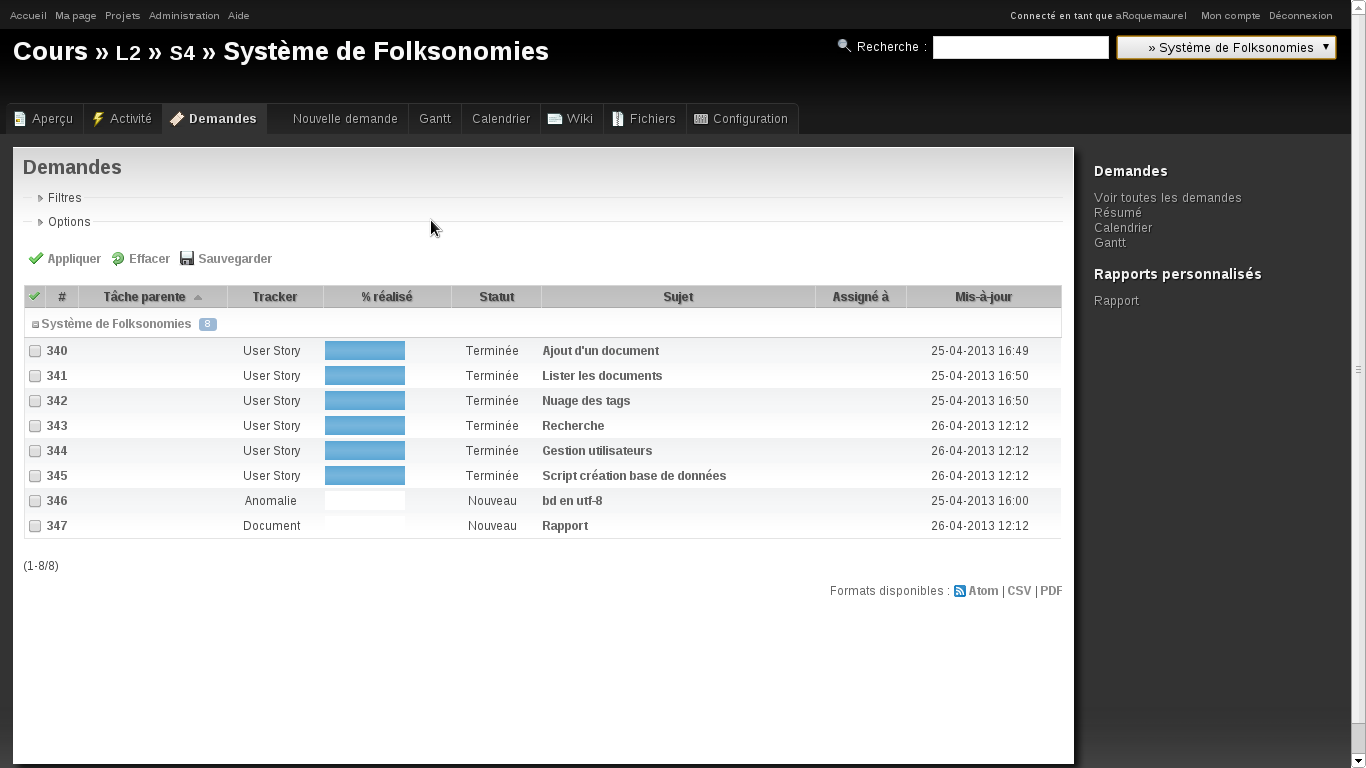
\includegraphics[width=18cm]{screens/redmine.png} %% TODO CHANGME
		\caption{Affichage des demandes dans Redmine}
		\label{fig:redmine}
	\end{figure}
	% TODO screen redmine
	Pour le projet, j'ai utilisé \textit{Redmine}, une plateforme web de gestion de projet (Cf figure \ref{fig:redmine}). Elle m'a permis 
	de simplifier le travail, et de ne rien oublier.

	En effet, je pouvais créer des tâches, signaler qu'elles sont en cours/terminés/en tests, leur donner des dates limites,
	etc\ldots 

	\section{Un logiciel de versionnement : Git}
	Afin de limiter les problèmes liés à une perte de données, j'ai utilisé un logiciel de versionnement Git. Il a deux intérêt, tout
	d'abord, je pouvais travailler de plusieurs ordinateurs en parallèle sur le projet sans me soucier de fusionner le travail\footnote{À condition de ne pas travailler sur deux lignes de code identiques}.

	D'autre part, tous les logs étant enregistrés, je pouvais voir l'avancée du projet. 

	Enfin, toutes les modification sont stockées sur le serveur, ainsi en cas de problème, il est très facile de revenir à la version précédente ou même de
	comparer deux versions afin de voir les changements et de comprendre rapidement pourquoi une fonctionnalité à régressé. 

	\chapter{Implémentation et conception}
		La conception du projet est l'étape la plus importante, ainsi j'ai préféré repenser à notre manière le projet, 
		je suis partis sur une architecture respectant le patron de conception MVC\footnote{Modèles Vue Contrôleur ou
		\textit{pattern MVC} : Model View Controller en anglais}, c'est à
		dire que toute la partie affichage (notamment le \bsc{HTML}), Modèle (c'est-à-dire les requêtes \bsc{SQL}) sont séparés, 
		c'est le Contrôleur qui dirige le modèle et la vue, c'est ainsi le \textit{chef d'orchestre}.
		\section{Mise en forme : les vues}
			Afin d'avoir un site web élégant sans passer beaucoup de temps à réinventer la roue en \bsc{CSS}, j'ai choisi d'utiliser un
			framework\footnote{Kit de composants logiciels structurels, qui sert à créer les fondations ainsi que les grandes lignes de tout ou d’une partie d'un
			logiciel (architecture). --- D'après \textit{wikipédia}} CSS
			appelé \bootstrap{}. Celui-ci nous permet d'avoir une mise en forme sobre très rapidement.  La mise en forme est organisé comme suit:

			\subsection{Le CSS} Le \bsc{css} est présent dans le dossier \texttt{style/css}, dedans est présent d'une part le
			\bsc{css} fourni par \bootstrap{}, auquel je n'ai pas touché, d'autre part, mon \bsc{css} qui surcharge certains affichage de \bootstrap{}, celui-ci est dans \texttt{style/css/style.css}.
			% TODO
			\lstinputlisting[language=CSS, caption=Exemple d'une partie du CSS]{code/css.css}
				
		\subsection{Le \bsc{HTML}}
		Le \bsc{html} correspond aux vues, tous les fichiers contenant du HTML sont dans le dossier \texttt{views/}, les formulaires 
		eux sont dans le dossier \texttt{views/forms}.
		
		Les vues peuvent ne comporter que du \bsc{html}, comme c'est le cas dans les formulaires, mais ils peuvent également comporter des instructions simples
		de \bsc{php} comme des boucles ou des conditions.

		Le dossier \texttt{views} contient également les fonctions d'affichage des documents ou une fonction permettant d'afficher une alerte. 
			\lstinputlisting[language=PHP, mathescape=false, caption=Fonction d'affichage d'une liste de documents]{code/documents.php}
		\section{Connexions à la base de données : Les modèles}
		L'application comporte trois modèles : un pour les documents, un pour les termes, et un pour les utilisateurs. Ces trois fichiers contiennent des fonctions effectuant des
		requêtes et retournant un tableau avec les attributs, ceci afin de bien séparer le \bsc{sql} du \bsc{php}.

		Également présent dans le dossier \texttt{database}, le fichier \texttt{connect.php} contient les identifiants et les
		instructions de connexion à la base de données. Le fichier \texttt{database.php} quant à lui contient les requêtes de
		création et suppression de la base.

		\lstinputlisting[language=SQL, mathescape=false, caption=Requête sélectionnant les documents d'un utilisateur donné ]{code/sql.sql}
		\lstinputlisting[language=PHP, mathescape=false, caption=Fonction d'insertion d'un document]{code/sql.php}
		\section{Liaison des vues aux modèles : Les contrôleurs}
		Chaque contrôleur correspond aux pages que verra un utilisateur lambda dans l'URL, les contrôleurs sont en général assez
		simples, ils font appels au modèle puis font une inclusion de la vue, ceux sont eux qui feront les éventuels vérifications
		sur des paramètres, sur une connexion pour l'insertion de document etc\ldots
		\lstinputlisting[language=PHP, mathescape=false, caption=Contrôleur de l'insertion d'un document]{code/controleur.php}
		Comme dit plus haut, c'est relativement simple, on inclus les vues et fonctions nécessaires, on vérifie qu'on a le droit
		d'être ici, on créer le tableau de mots clés, puis on insère le tout e faisant appel au modèle.

	\chapter{Résultats obtenus}
	Dans cette partie, nous allons regrouper quelques captures d'écrans montrant les résultats obtenus sur notre application Web.
	L'application est répartie en 3 fonctionnalités principales : 
	\begin{itemize}
		\item L'affichage des séries et épisodes présents
		\item La recherche de série ou épisodes
		\item L'ajout de série ou épisodes
	\end{itemize}
	L'ajout d'épisodes implique la possibilité de se connecter afin que seul l'administrateur puisse utiliser l'administration.
	\remarque{Le couple login/mot de passe de l'application est admin/admin}
	\section{Affichage des séries et épisodes}
	\begin{figure}[H]
		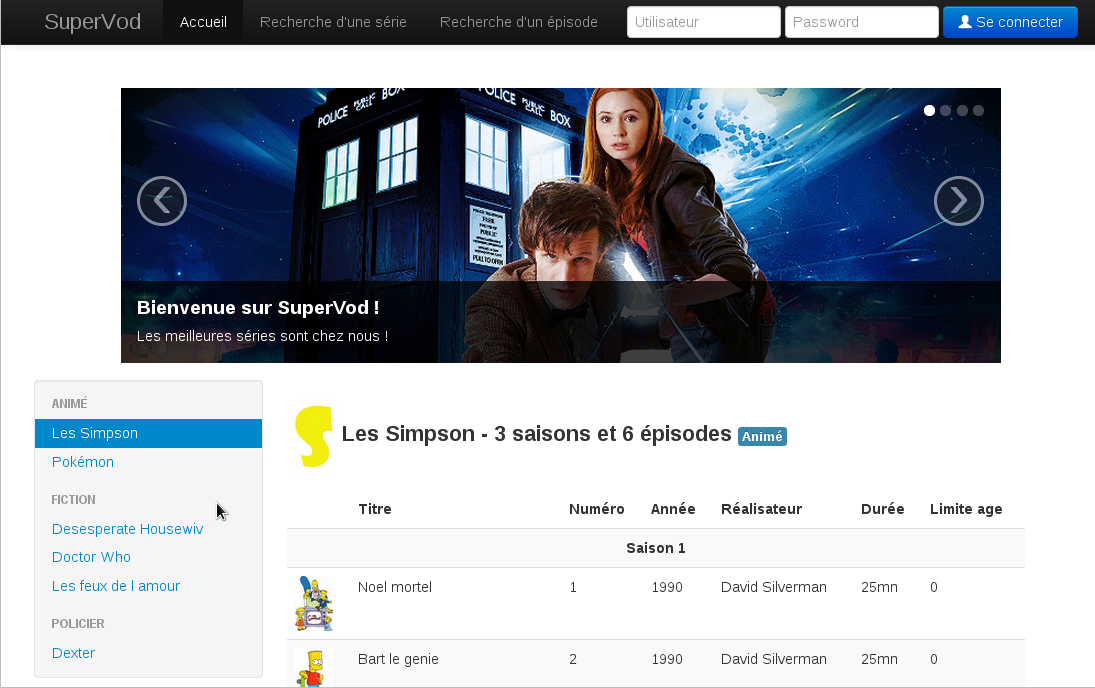
\includegraphics[width=18.0cm]{screens/accueil.png}
		\caption{Page d'accueil de l'application}
		\label{fig:accueil}
	\end{figure}
	La figure \ref{fig:accueil} nous montre la page d'accueil du site, avec la possibilité de sélectionner une série via le menu de gauche, affichant ainsi tous
	ses épisodes. On peut remarquer sur cette figure que le site possède un thème qui est commun à tout le site : la barre de navigation en haut de l'écran
	permet d'accéder d'un clique à chacune des fonctionnalités présentes sur le site.
	\section{Recherche}
	\begin{figure}[H]
		\centering
		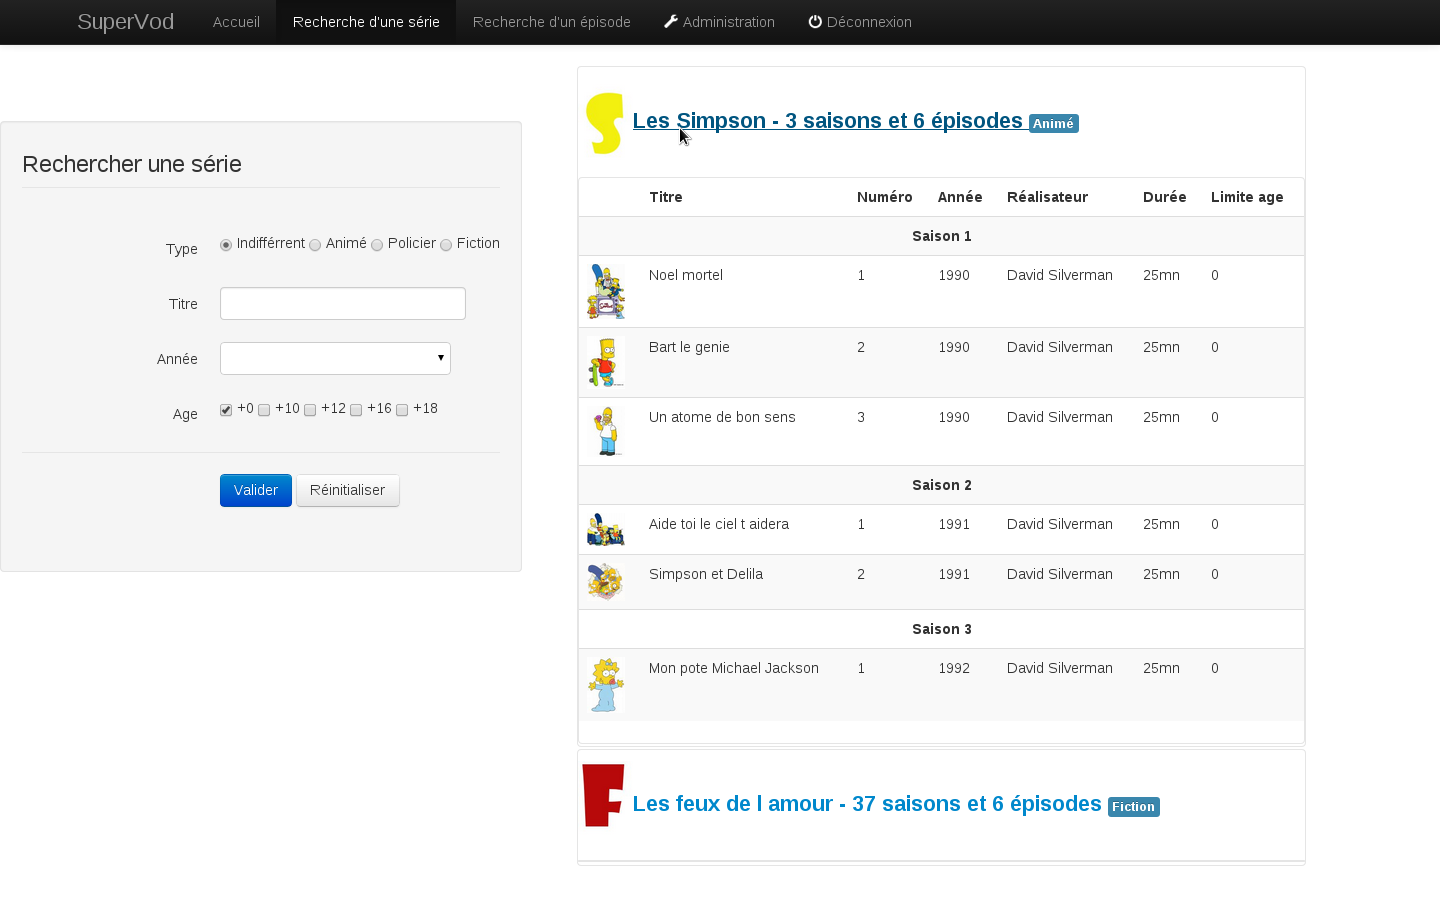
\includegraphics[width=15.7cm]{screens/rechercheSerie.png}
		\caption{Recherche d'une série}
		\label{fig:rechercheSerie}
	\end{figure}
	\begin{figure}[H]
		\centering
		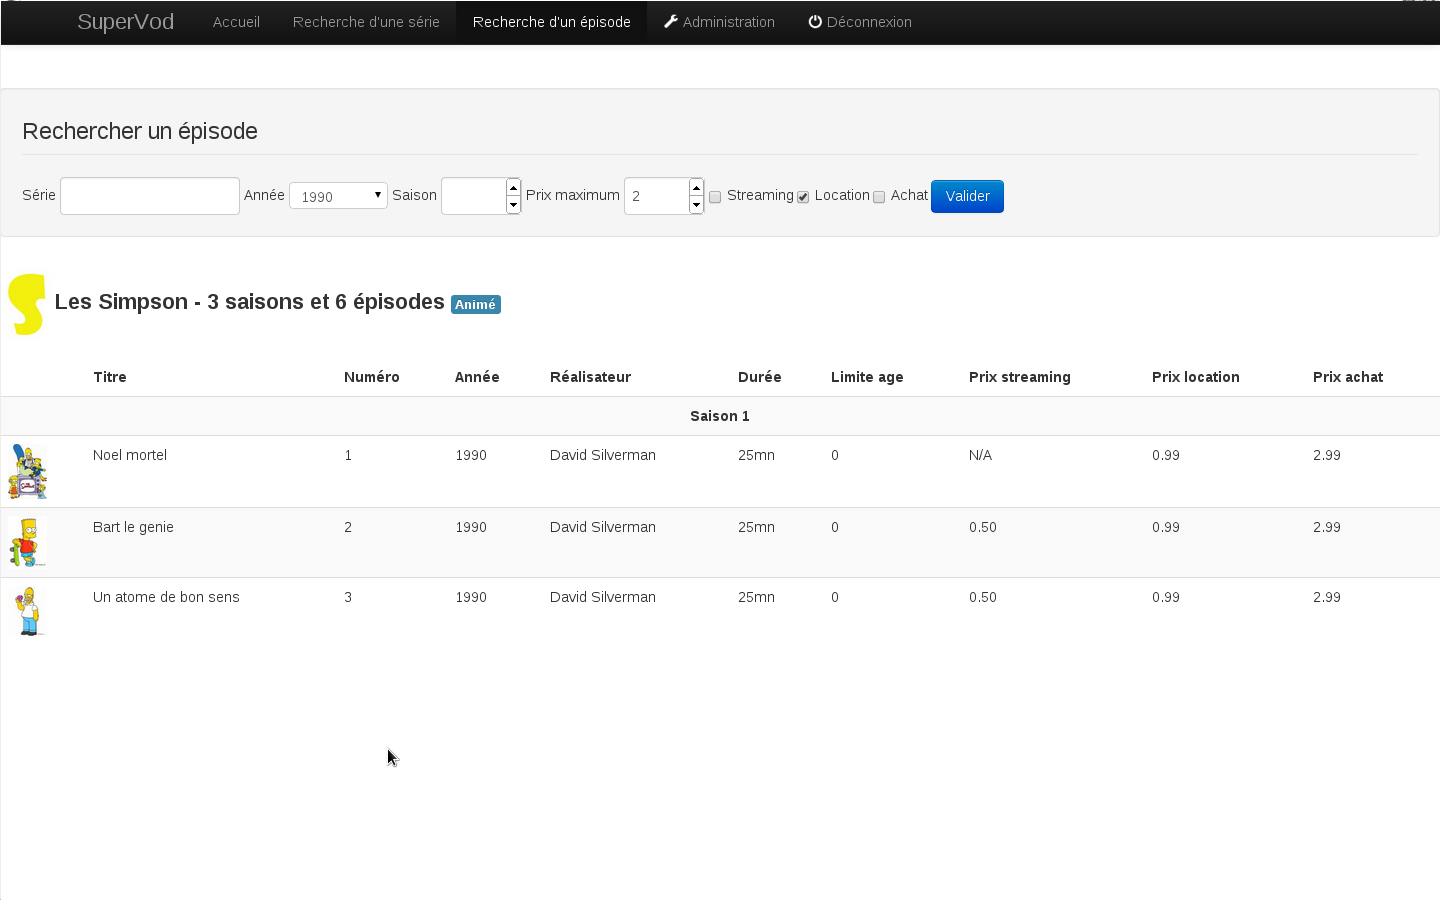
\includegraphics[width=15.7cm]{screens/rechercheEpisodes.png}
		\caption{Recherche d'un épisode}
		\label{fig:rechercheEpisode}
	\end{figure}
	Les figures \ref{fig:rechercheSerie} et \ref{fig:rechercheEpisode} nous montrent respectivement la recherche d'une série et la recherche d'un épisode.

	Ces deux fonctionnalités sont assez similaires, bien que les critères de recherches soit différents. Ainsi, la recherche d'une série affiche les séries
	répondants au critères renseignés\footnote{Une série peut être cherché par son type, son titre, ses années de diffusion ainsi que son age}, ainsi que la
	possibilité d'affiche les épisodes correspondants de la série.

	La recherche d'un épisode quand à elle à une mise en forme différente, étant donné qu'il y a plus d'informations a afficher pour un épisode, cependant le
	principe reste le même via les critères de recherche\footnote{Un épisode peut être trouvé grâce à sa série, son année de diffusion, sa saison, le prix
	maximum auquel on veut l'acheter, ainsi que sa disponibilité (Streaming, Location, Achat)}
	\section{Ajout de séries et épisodes}
	\begin{figure}[H]
		\centering
		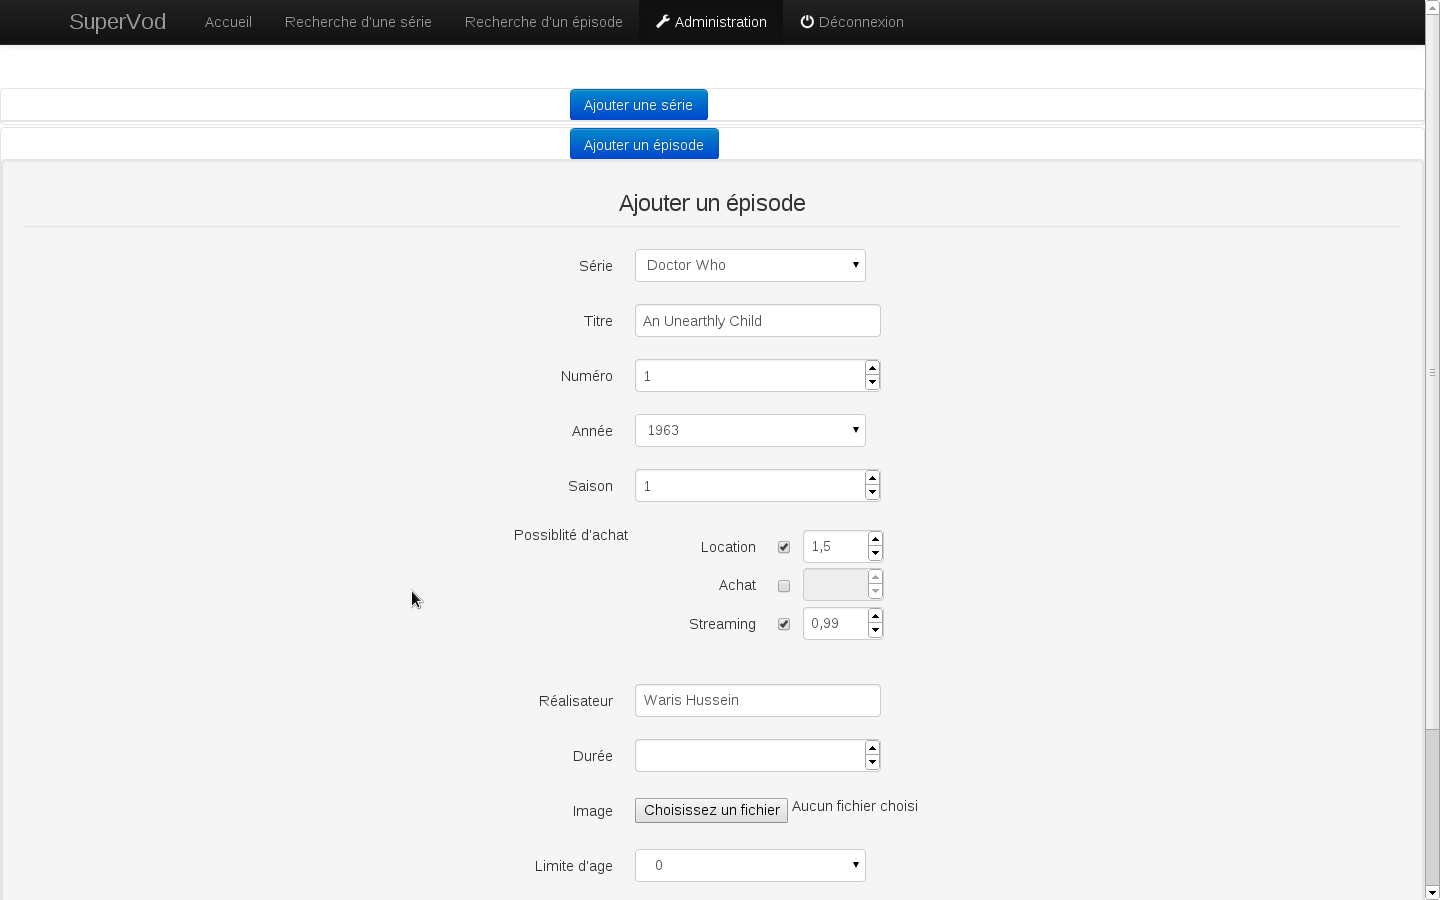
\includegraphics[width=18.5cm]{screens/adminEpisode.png}
		\caption{Administration}
		\label{fig:admin}
	\end{figure}
	La figure \ref{fig:admin} nous montre la partie administration, ici l'ajout d'un nouvel épisode à la série \textit{Doctor Who}, tous les champs présents
	précédemment peuvent être renseignés, cependant seuls les champs Série, Titre, Numéro et Saison sont obligatoires, les autres sont facultatifs.\\
	Il est également possible de sélectionner une image pour la série depuis notre ordinateur via un champ d'upload.

	Nous n'avons pas fait de capture d'écrans de l'ajout d'une série, cependant le principe est le même bien que les champs soient moins nombreux, pour une
	série, les champs Type et Nom sont obligatoires.
	\section{Valide HTML5}
	\begin{figure}[H]
		\centering
		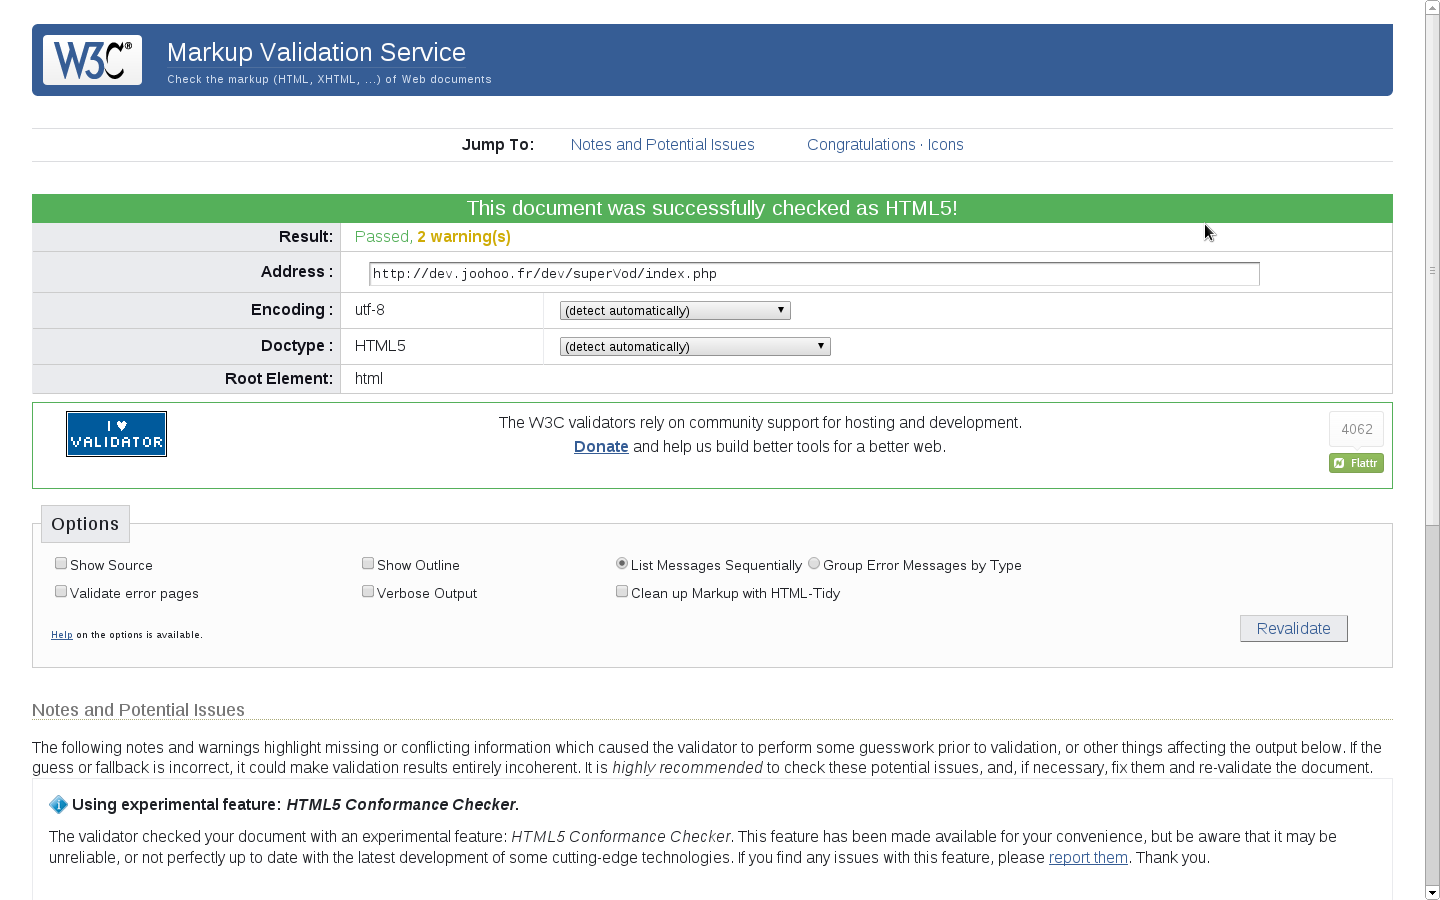
\includegraphics[width=17cm]{screens/htmlValidator.png}
		\caption{HTML5 validator -- Passed}
		\label{fig:htmlValidator}
	\end{figure}
	La figure \ref{fig:htmlValidator} montre simplement notre site web passant la validation du \bsc{w3c}\footnote{World Wide Web Consortium} avec la norme
	HTML5.
	\appendix
	\listoffigures
	\removepagebreak
	\vfill
	\lstlistoflistings
	\vfill
	\restorepagebreak
\end{document}

